%%This is a very basic article template.
%%There is just one section and two subsections.
\documentclass[a4paper, ngerman]{scrartcl}

\usepackage[T1]{fontenc}
\usepackage[utf8]{inputenc}
\usepackage[ngerman]{babel}
\usepackage{lmodern}
\usepackage{amsmath}
\usepackage{amsfonts}
\usepackage{hyperref}
\usepackage{graphicx}
\usepackage{paralist}
\usepackage[none]{hyphenat}

\sloppy



\hypersetup{ 
pdfborder = {0 0 0}, 
urlbordercolor = {0 0 0}, 
colorlinks = true,
linkcolor = black,
citecolor = black,
filecolor = black,
urlcolor  = black
}

\title{Software-Challenge 2015 \\ Hey, danke für den Fisch}
\subtitle{Spielregeln}



%% Variablen
\newcommand{\FelderAnzahl}{\emph{60}}
%%\newcommand{\KartenAnzahl}{\emph{KartenAnzahl}}
\newcommand{\PinguinAnzahl}{\emph{4}}
\newcommand{\EmptyPlainPage}{\newpage\thispagestyle{plain}\ \newpage}
\newcommand{\RundenAnzahl}{\emph{56}}

\begin{document}
\parindent0px
\maketitle

\begin{figure}[h!]
	\centering
	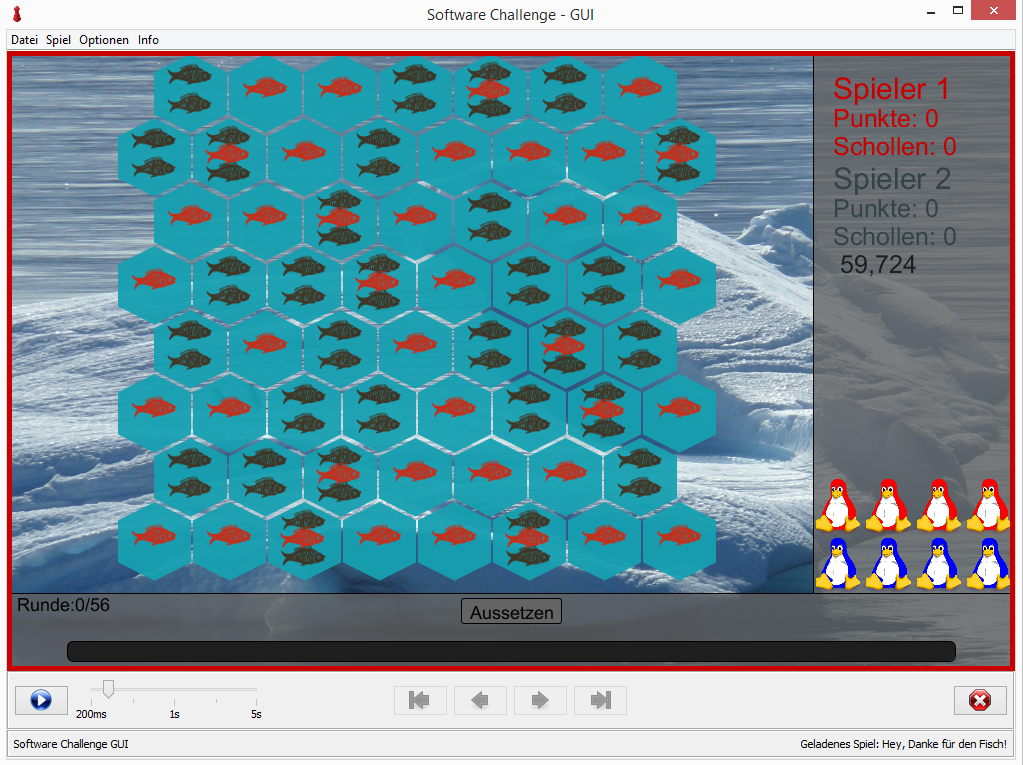
\includegraphics[width=\linewidth]{bilder/gui.png} 
\end{figure}
\vspace*{\fill}
"Die Nutzung des Spielkonzeptes "Hey, danke für den Fisch" (Name, Spielregeln
und Grafik) erfolgt mit freundlicher Genehmigung des Heidelberger
Spieleverlags."
\newpage
\tableofcontents
\newpage

\section{Einführung}
In dieser Anleitung werden die Elemente und Regeln des Spiels \emph{Hey, danke
für den Fisch} der Software-Challenge 2015 erläutert.\\
Zu Beginn des Spiels setzt zunächst Rot einen Pinguin auf eine unbesetzte Scholle mit nur einem Fisch. Danach tut Blau das Gleiche. So wechseln sich die Spieler ab, bis alle Pinguine auf dem Spielfeld verteilt sind.
Anschließend versuchen die beiden Spieler abwechselnd – Blau zuerst – einen eigenen Pinguin auf eine unbesetzte Scholle zu ziehen und dabei möglichst viele Fische einzusammeln.

\section{Spielmaterial}
	\subsection{Das Spielbrett}
Das Spielbrett setzt sich aus 60 sechseckigen Schollen zusammen,
mit jeweils einem, zwei oder drei Fischen.
Die Verteilung der 30 Schollen mit einem Fisch, 20 mit zweien und 10 mit
dreien ist zufällig.
Jede gerade Reihe hat hierbei jeweils 7 Schollen und jede ungerade 8
Schollen, wobei die oberste Reihe die Reihe Null ist. Ein mögliches
Spielbrett ist in Abbildungen 1-3 zu sehen.
\section{Spielablauf}	 

	%% an Beispiel erklären
	Es beginnt der rote Spieler. Jeder Spieler darf abwechselnd einen
	Zug machen. Innerhalb der ersten 4 Runden sind nur Setzzüge möglich. Ab der
	5.
	Runde sind beginnend mit dem blauen Spieler nur noch Laufzüge möglich.\\
	Sobald ein Spieler eine Figur ausgewählt hat, werden sämtliche Felder, auf
	welche die Figur ziehen kann, farbig markiert.
	 
	
	
	\subsection{Setzzüge}
	
	\begin{figure}[h!]
		\centering
		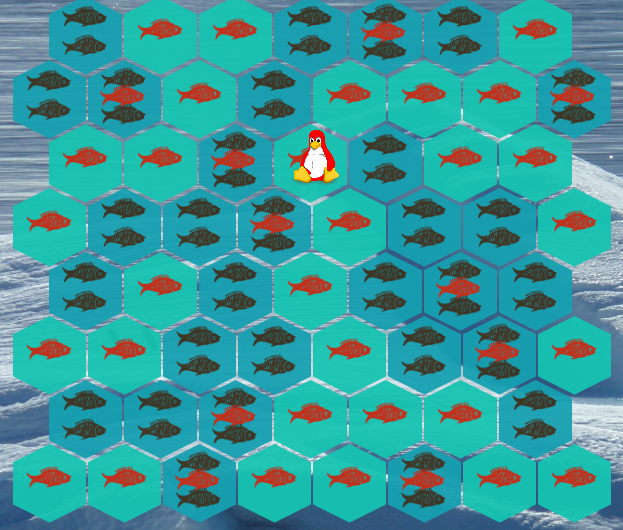
\includegraphics[scale = 0.4]{bilder/setzzug.png}
		\caption{Spielsituation in der Setzphase.}
		\label{fig:Setzzug}
	\end{figure}
	%% an Beispiel erklären
	Bei einem Setzzug wählt ein Spieler einen seiner
	Pinguine und zieht ihn auf eine Scholle ohne Pinguin, auf der sich nur ein
	Fisch befindet.\\
	Bei einem Setzzug kann nicht ausgesetzt werden. Durch gedrückthalten der Maus
	wird ein Pinguin gezogen und durch loslassen auf das jeweilige Spielfeld
	gesetzt.
	
	
	 
\subsection{Laufzüge}
	 
	\begin{figure}[h!]
		\centering
		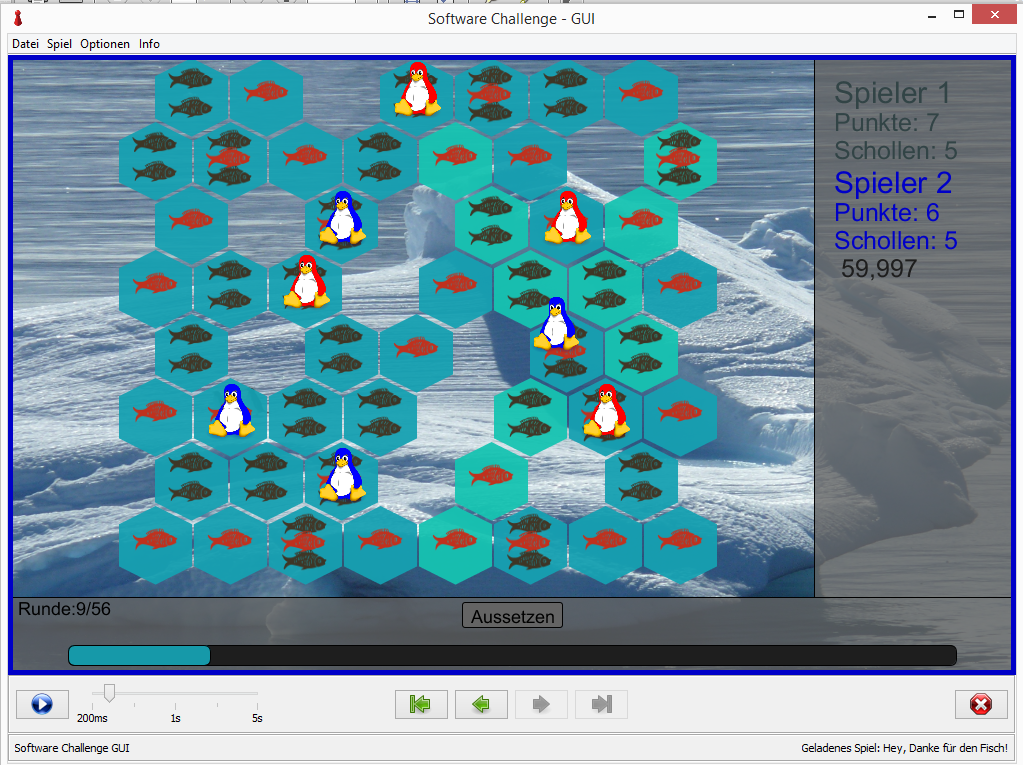
\includegraphics[scale=0.4]{bilder/laufzug.png}
		\caption{Eine Spielsituation in der Laufzugphase.}
		\label{fig:Laufzug}
	\end{figure}
	
%% an Beispiel erklären
Ab derder 5. Runde sind Laufzüge möglich. Bei einem Laufzug
ist es möglich, einen Pinguin entweder entlang der Horizantalen oder der beiden
Diagonalen zu bewegen. Ein Pinguin kann hierbei nicht über oder auf Löcher oder
andere Pinguine ziehen. Die vom Pinguin verlassene Scholle wird vom Spielfeld entfernt.
Die Fische auf dieser Scholle werden zum Fischdepot des Spielers addiert und sein 
Schollendepot wird um 1 erhöht.



\subsection{Aussetzzüge}
%% an Beispiel erklären 
Ein Aussetzzug ist an Stelle eines Laufzugs möglich. Dieser ist normalerweise
nur dann sinnvoll, wenn kein anderer Zug möglich ist.

	
\section{Ende des Spiels} 
	Das Spiel endet, sobald beide Spieler nur noch aussetzen können, 
	spätestens jedoch nach 30 Runden.  Beim Spielende bekommt jeder 
	Spieler noch die Fische, auf denen seine Pinguine dann stehen, 
	auf seinem Fischdepot gutgeschrieben und sein Schollendepot wird 
	je eigenem Pinguin um 1 erhöht.
	Das Spiel gewinnt der Spieler mit den meisten Fischen. Bei Gleichstand gewinnt
	der Spieler mit den meisten Schollen. Herrscht auch dort Gleichstand, endet das
	Spiel unentschieden.
	
\section{Die graphische Benutzeroberfläche}
\subsection{Graphischen Benutzeroberfläche}
	In Abbildung~\ref{fig:GUI} ist ein Überblick der graphischen Benutzeroberfläche
	zu sehen. Die markanten Spielelemente sind mit \emph{A-E} gekennzeichnet.
	
	 \begin{figure}[h!]
		\centering		
		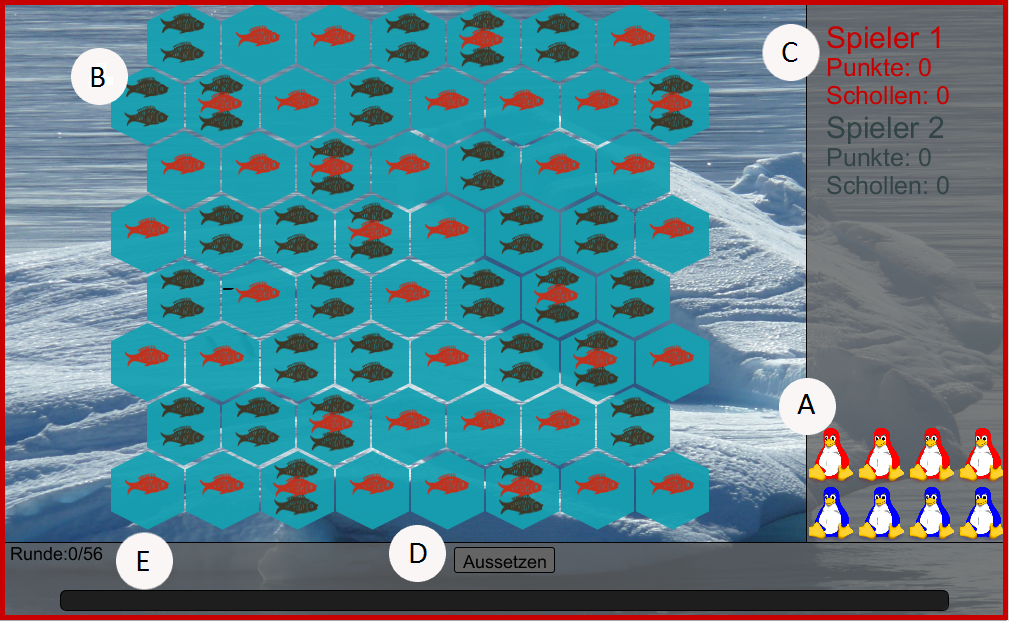
\includegraphics[scale = 0.5]{bilder/uebersicht.png} 
		\caption{Überblick der GUI}
		\label{fig:GUI}
	\end{figure} 
	%% wie ist die Benutzeroberfläche?
\begin{compactenum}[A)] 
\item Die Pinguine befinden sich anfangs rechts.
\item Das Spielbrett  
\item Fischdepot.
 Die Fische und Schollen des roten Spielers sind 
oben, die des blauen Spielers unten. Die Fische des inaktiven Spielers sind
jeweils in grau dargestellt.
\item Der Aussetzknopf
\item  Die Spielfortschrittsanzeige
	\end{compactenum}
	
\subsection{Das Einstellungsmenü} 
	 \begin{figure}[h!]
		\centering
		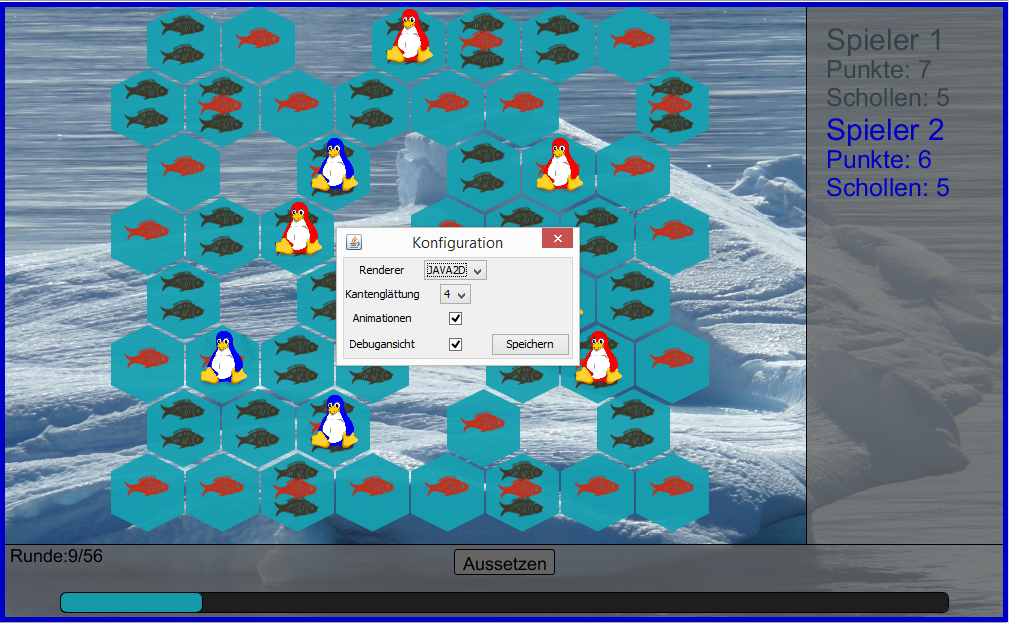
\includegraphics[scale=0.4]{bilder/konfiguration.png}
		\caption{Das Einstellungsmenü}
		\label{fig:Configuration}
	\end{figure}
	
	Ein Einstellungsmenü mit Darstellungsoptionen lässt
sich über die Taste 'C' anzeigen. Dazu muss das
Spielfeld den Tastaturfokus haben (erforderlichenfalls
vorher Mausklick auf das Spielfeld). Es stehen dort
folgende Einstellungen zur Verfügung: 

\textbf{Kantenglättung} verbessert die Optik des
Spiels, ist aber rechenintensiv. Auf sehr langsamen Rechnern sollten sie daher
deaktiviert werden.
\textbf{Animationen} legt fest, ob die Bewegungen der Spielsteine in
Wiederholungen und bei Computerspielern animiert werden sollen.\\
Die \textbf{Debugansicht} zeigt Debug-Hilfestellungen zu einzelnen Zügen und
die Framerate an.
Diese Hilfestellungen sind Texte, die ein Spielclient einem Zug beifügen kann, den er
an den Spielserver sendet.
	
\end{document}
